\section{Conception Matérielle}
Pour mettre en oeuvre les différentes parties du projet combinatoires et séquentielles, nous avons du passer par des étapes d'analyses comportementales de chaque blocs à réaliser pour ainsi créer des composants simples pouvant être utiliser à la composition de fonctions plus complexes plus tard. L'implémentation de chaque composants a été réalisée grâce au langage VHDL sur le logiciel de développement Quartus.

Ainsi nous avons réalisé différentes "boîtes" de composants simples pour réaliser des fonctions entières, et plus complexes, contenant les blocs simples.

\subsection{Réalisation fonction simple - Gestion anémomètre}
La fonction réalisant l'acquisition de la vitesse du vent (0 à 250 Km/h) se fait à l'aide d'un anémomètre qui sert de transducteur convertissant la vitesse du vent en fréquence variable (0 à 250 Hz). 
\vspace{0.5cm}\\
Le composant doit fonctionner en deux modes :
\begin{enumerate}
    \item Mode continu, dans ce mode le système actualise l'acquisition toutes les secondes de la vitesse du vent.  
    \item Mode mono-coup, dans ce mode le système effectue qu'une seule acquisition lorsque "Start/stop" est activé. Une fois "data\_valide" envoyé le système remet les entrées "start/stop" et "data\_valide" à zéro après une acquisition.
\end{enumerate}
\vspace{0.5cm}
La figure 3 représente la décomposition des composants utilisés pour la réalisation du bloc "Captage direction vent". Composé d'un diviseur de fréquence (pour obtenir une fréquence d'un Hertz, acquisition toutes les sécondes), d'un détecteur de fronts montants (permettant d'indiquer le nombre de fronts montants correspondant à la fréquence mesurée), d'une machine à état (pour décrire séquentiellement les modes continu/mono-coup), un compteur (pour l'acquisition du nombre de fronts montants toutes les secondes) et une Bascule D (permettant la mémorisation de la valeur et l'acquisition avant obtention de la nouvelle valeur).

\begin{figure}[h]
    \begin{center}
      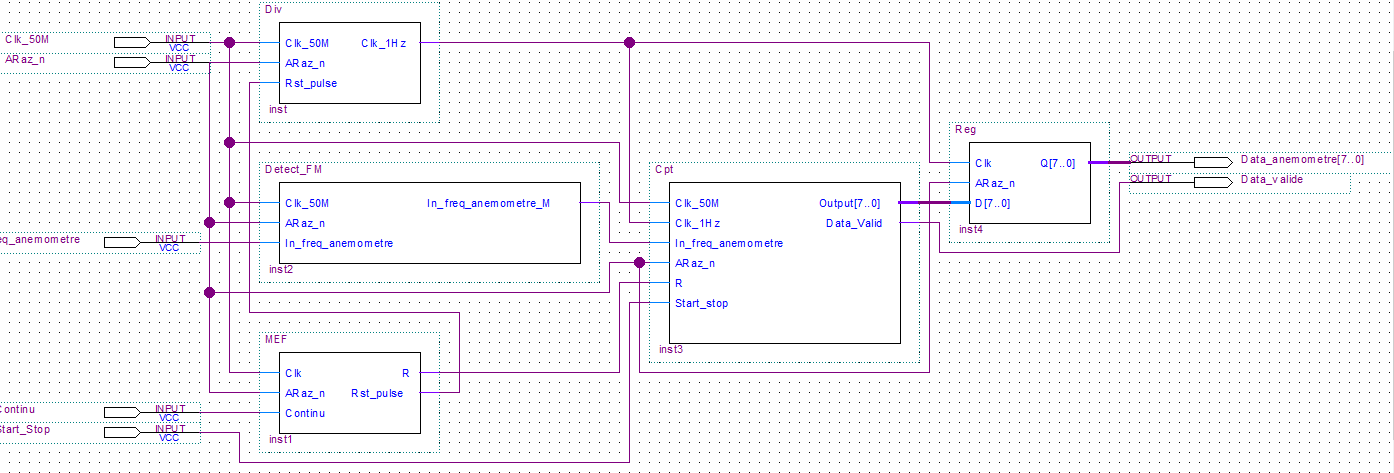
\includegraphics[width=\textwidth]{images/captation.png}
      \caption{Diagramme fonctionnel du circuit "Captation vitesse vent"}
    \end{center}
  \end{figure}

  \newpage

  \subsection{Réalisation fonction complexe - Gestion vérin}